\documentclass{article}%
\usepackage[T1]{fontenc}%
\usepackage[utf8]{inputenc}%
\usepackage{lmodern}%
\usepackage{textcomp}%
\usepackage{lastpage}%
\usepackage[head=40pt,margin=0.5in,bottom=0.6in]{geometry}%
\usepackage{graphicx}%
%
\title{\textbf{La OMS señala que sistema sanitario venezolano se redujo 20\%}}%
\author{EFE}%
\date{03/12/2018}%
%
\begin{document}%
\normalsize%
\maketitle%
\textbf{URL: }%
http://www.el{-}nacional.com/noticias/mundo/oms{-}senala{-}que{-}sistema{-}sanitario{-}venezolano{-}redujo\_261993\newline%
%
\textbf{Periodico: }%
EN, %
ID: %
261993, %
Seccion: %
Mundo\newline%
%
\textbf{Palabras Claves: }%
NO\_TIENE\newline%
%
\textbf{Derecho: }%
2.1, %
Otros Derechos: %
18, %
Sub Derechos: %
2.1.1\newline%
%
\textbf{EP: }%
NO\newline%
\newline%
%
\textbf{\textit{El director general de la Organización Mundial de la Salud (OMS), Tedros Adhanom Ghebreyesus, recordó que Venezuela ha sufrido un incremento de enfermedades como el sarampión, la difteria y la malaria~}}%
\newline%
\newline%
%
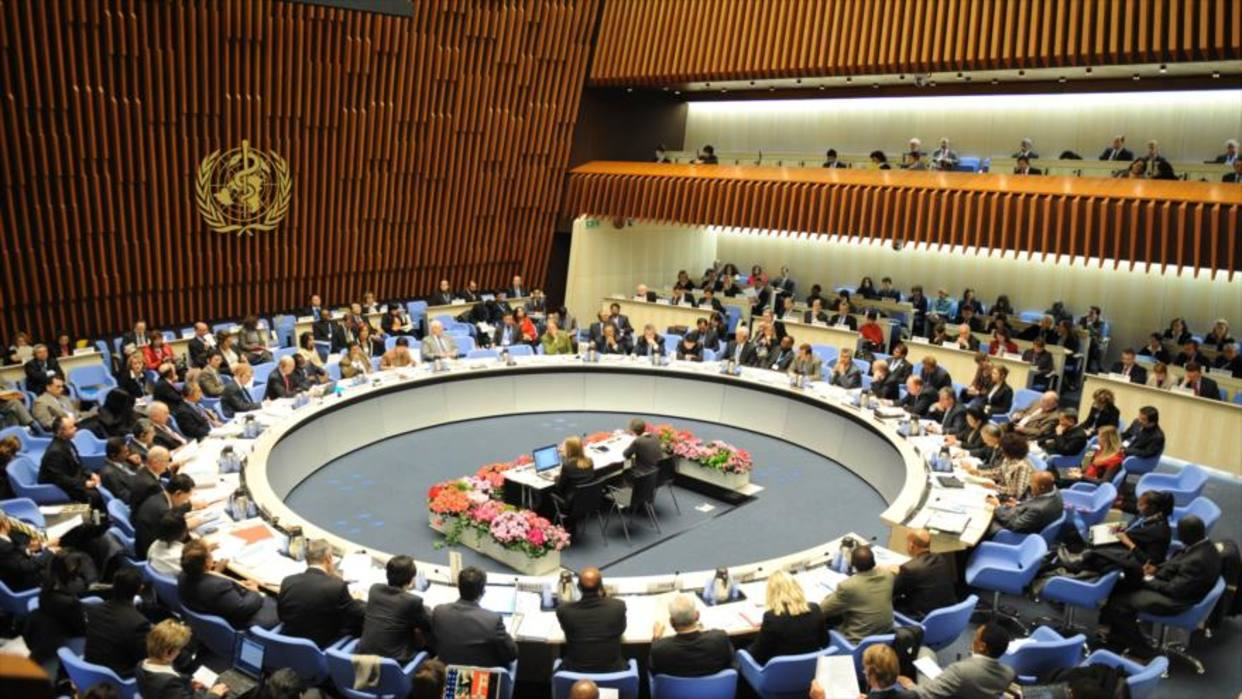
\includegraphics[width=300px]{78.jpg}%
\newline%
%
La crisis que vive Venezuela en los últimos años ha reducido entre 15 y ~20 \% la capacidad de atención médica en el país, admitió hoy el director general de la Organización Mundial de la Salud (OMS), Tedros Adhanom Ghebreyesus, en rueda de prensa.%
\newline%
%
"Estimamos que los servicios de salud se han reducido al 80{-}85 por ciento, con muchos médicos y enfermeras que han abandonado el país", subrayó Tedros tras afirmar que Venezuela afronta dificultades sociales, políticas y económicas.%
\newline%
%
El máximo responsable de la OMS también recordó que el territorio venezolano ha sufrido un incremento de enfermedades como el sarampión, la difteria y la malaria, frente al cual el organismo internacional está intentando cooperar con el gobierno de Nicolás Maduro mediante asistencia técnica y campañas de vacunación.%
\newline%
%
"Al mismo tiempo estamos trabajando con países vecinos como Colombia, Brasil, Perú o Ecuador, receptores de refugiados (venezolanos), para intentar que esas carencias en servicios sanitarios sean subsanadas", añadió Tedros.%
\newline%
%
Naciones Unidas anunció la semana pasada que su Fondo Central de Respuesta a Emergencias destinará 9,2 millones de dólares a programas de asistencia nutricional a grupos de riesgo y de ayuda sanitaria de emergencia en Venezuela.%
\newline%
%
Tedros declinó hoy dar detalles sobre esta asistencia y tampoco confirmó el grado de implicación de la OMS en estos programas, que suponen el primer envío de ayuda humanitaria de la ONU al régimen de Maduro, que durante largo tiempo se ha resistido a reconocer que su país vivía una crisis humanitaria.%
\newline%
%
\end{document}